\documentclass[tikz]{standalone}

\usepackage{tikz}
\usepackage{xcolor}
\usepackage{pgfplots}
\usepackage{../tikzviolinplots}
%\usepgfplotslibrary{external}
%\tikzexternalize
\usepackage{siunitx}
\usepackage{fontspec}

\pgfplotsset{compat=1.18}
\setmainfont{Source Serif 4}[
    Renderer = OpenType,
    SizeFeatures    = {%
        {Size={-9},Font=* Caption},
        {Size={9-13},Font=*},
        {Size={14-24},Font=* Subhead},
        {Size={24-},Font=* Display}
    },
    ItalicFeatures = {%
    SizeFeatures    = {%
            {Size={-9},Font=* Caption Italic},
            {Size={9-13},Font=* Italic},
            {Size={14-24},Font=* Subhead Italic},
            {Size={24-},Font=* Display Italic}
    },
    },
    BoldFeatures = {%
    SizeFeatures    = {%
            {Size={-9},Font=* Caption Semibold},
            {Size={9-13},Font=* Semibold},
            {Size={14-24},Font=* Subhead Semibold},
            {Size={24-},Font=* Display Semibold}
    },
    },
    BoldItalicFeatures = {%
    SizeFeatures    = {%
            {Size={-9},Font=* Caption Semibold Italic},
            {Size={9-13},Font=* Semibold Italic},
            {Size={14-24},Font=* Subhead Semibold Italic},
            {Size={24-},Font=* Display Semibold Italic}
    },
    },
    Numbers         = OldStyle,
]

\usetikzlibrary{shapes,arrows,positioning,backgrounds,calc,intersections,calc,svg.path,fit,fpu}
\definecolor{ugent-re}{RGB}{220, 78, 40}        % vermilion			/ vermiljoen
\definecolor{ugent-we}{RGB}{45, 140, 168}       % no match

\begin{document}
\begin{filecontents}[overwrite]{violin-large.dat}
    A,B,C,D,E
    -0.0008,0.002,0.0045,0.0066,0.0112
    -0.0025,0.0145,0.0278,0.0454,0.0764
    -0.0228,0.0107,0.0324,0.0622,0.107
    -0.5291,-0.167,0.0568,0.2965,0.6242
    -0.0671,-0.0532,-0.0528,-0.0568,-0.1213
    -0.0016,0.0029,0.0057,0.0093,0.0148
    -0.2582,-0.0385,0.0917,0.2522,0.4371
    -3.7579,-2.4503,-2.0196,-1.0449,-0.4214
    -0.051,-0.0184,-0.0003,-0.0002,0.001
    -1.0027,-0.338,-0.5583,-0.633,-0.8617
    -0.0318,0.0015,0.0047,-0.0388,-0.0274
    -10.2283,-6.7521,-6.7599,-4.6477,-3.1011
    -0.0004,0.0003,0.0003,0.001,0.001
    -0.0023,0.0036,0.0051,0.0102,0.0417
    -3.5335,0.9119,-1.3041,0.2481,1.2299
    0.0028,0.0027,0.0014,0.0021,0.0035
    0.0048,0.0473,0.0687,0.1002,0.1104
    -0.0388,0.0045,0.1639,0.179,0.0582
    -1.2101,-1.0269,-0.8964,-0.9092,-0.8266
    -0.0817,-0.0685,-0.0236,-0.0585,-0.0491
    -22.1854,-24.8918,-23.7397,-25.1552,-30.2728
    -2.3147,-1.774,-1.4241,-1.3589,-1.1706
    -0.0191,0.3992,0.8545,0.8075,1.1448
    -0.0146,-0.0079,-0.0001,0.0039,0.0056
    -0.1011,-0.0671,-0.0272,-0.0242,-0.0121
\end{filecontents}
\begin{tikzpicture}
    \pgfplotsset{height=5cm,width=6cm}
    \pgfkeys{/pgfplots/yticklabel={\addfontfeature{Numbers={Lining}}\qty[round-mode=places, round-precision=0]{\tick}{\mega{}}},}
    \violinsetoptions[
        scaled,
        averages,
    ]{
        xmin=0.3,xmax=6.2,
        ymin=-45,ymax=15,
        xlabel style={
            yshift = {-3*height("a")}
        },
        ymajorgrids=true,
        ytick distance=10,
        ylabel={№ of blocks}
    }
    \violinplot[%
        index=A,
        relative position=1,
        label={30},
        samples=100,
        average mark=*,
        average fill=black,
        average fill opacity=1.0,
        average size=1pt,
        color=ugent-we,
    ]{violin-large.dat}
    \violinplot[%
        index=B,
        relative position=2.2,
        label={60},
        samples=100,
        average mark=*,
        average fill=black,
        average fill opacity=1.0,
        average size=1pt,
        color=ugent-we,
    ]{violin-large.dat}
    \violinplot[%
        index=C,
        relative position=3.3,
        label={90},
        samples=100,
        average mark=*,
        average fill=black,
        average fill opacity=1.0,
        average size=1pt,
        color=ugent-we,
    ]{violin-large.dat}
    \violinplot[%
        index=D,
        relative position=4.4,
        label={120},
        samples=100,
        average mark=*,
        average fill=black,
        average fill opacity=1.0,
        average size=1pt,
        color=ugent-we,
    ]{violin-large.dat}
    %! parser = off
    \pgfkeys{
        /pgfplots/xticklabels={\addfontfeature{Numbers={OldStyle,Proportional}}\textsc{asap}},
        /pgfplots/xlabel={Execution models (\textsc{em-})},
    };
    %! parser = on
    \violinplot[%
        index=E,
        relative position=5.5,
        samples=100,
        average mark=*,
        average fill=black,
        average fill opacity=1.0,
        average size=1pt,
    ]{violin-large.dat}
\end{tikzpicture}
\end{document}
